\section{Data}
The main input of the Article/Editors ranking algorithm is the matrix $M$ which determines, for a category on Wikipedia, which articles have modified at least once by each editor. We collected contribution data for articles in 10 categories (c.f. table \ref{tab:statistics} for summary statistics on the categories). In addition, we made 10 snapshots of equal number of edits to account for the evolution over time of each category (see Figure \ref{fig:accumulative_snapshots}
).

\begin{tabular}{llll}
\toprule
Category & Users & Articles &  Edits \\
\midrule
2013 films &  5215 &     1896 &  150956 \\
American male novelists &  9946 &     2460 &  224783 \\
American women novelists &  5968 &     1936 &  138716 \\
Bicycle parts &   210 &       70 &    4981 \\
Computability theory &   272 &       92 &    7117 \\
Counterculture festivals &   578 &       66 &   10515 \\
Economic theories &  1145 &      212 &   28658 \\
Feminist writers &  1357 &      233 &   25738 \\
Military history of the US &   854 &      180 &   20172 \\
Nobel Peace Prize laureates &  4165 &      104 &   91522 \\
Sexual acts &  2190 &       93 &   45901 \\
Yoga &   730 &      123 &   25315 \\
\bottomrule
\label{tab:statistics}
\end{tabular}

\begin{figure}[!t]
\centering
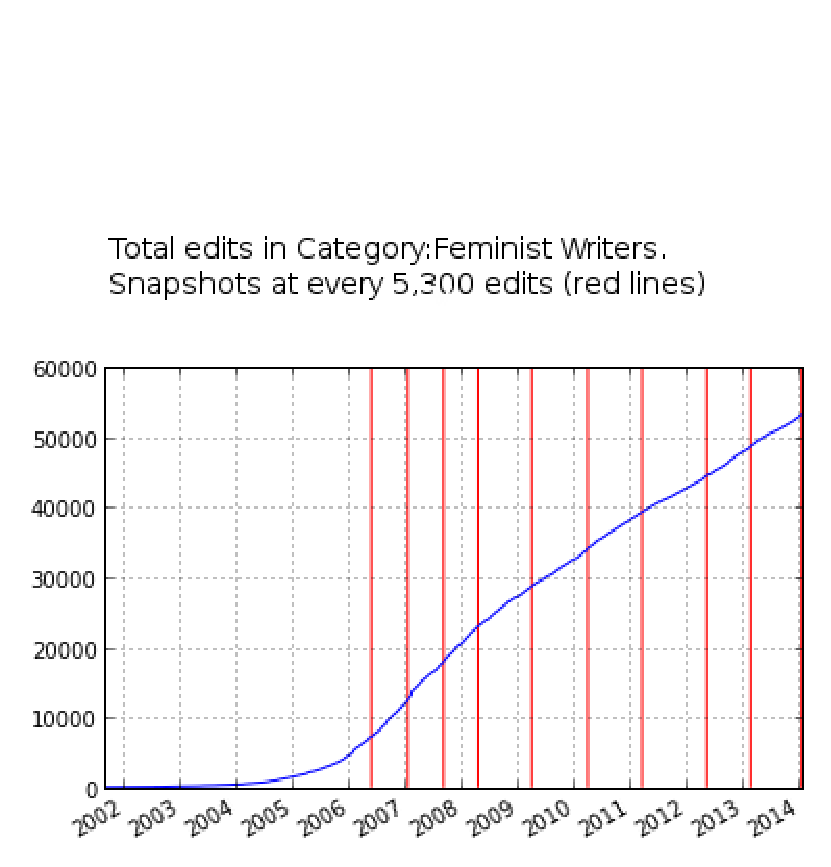
\includegraphics[width=0.9\columnwidth]{Figures/cumulative_snapshots_Feminist_Writers.eps}
\caption{cumulative snapshots Feminist Writers eps }
\label{fig:figure1}
\end{figure}

 For each snapshot, we constructed the matrix $\mathbf{M_{e,a}}$ of contributors versus edited articles, similar to the country versus products matrix of the Economics Domain. For each snapshot, the values in $\mathbf{M_{e,a}}$ are defined as the number of edits made by editor $e$ on article $a$ in the category occurring in the snapshot time. Note that the final snapshot represents the entire history of the category up to the present date.
  
The matrix $\mathbf{\hat{M}_{e,a}}$ is a binary representation of $\mathbf{M_{e,a}}$ where each nonzero entry is replaced with $1$. This represents if editors have touched which articles rather than how much they have touched each article. In the economics domain, the distinction of making a binary matrix out of the data is interpreted an alternative metric to GDP per capita, rather than GDP. Here we could also see the distinction as normalized editor fitness. It has a typical triangular structure as shown on Figure \ref{fig:triangular_matrix}. The matrix $\mathbf{\hat{M}_{e,a}}$ constitutes the basic input for implementing the Biased Markov Chain Approach, which we will call the $\mathbf{w^*}$ algorithm, which is an analytic solution to the iterative $\mathbf{W}$ algorithm. \cite{Caldarelli} 

The exogenous metric for editors $v_e$ we take is $labour hours$. For each editor the contribution history upto the snapshot point,  divide into strings of $edit sessions$, edits that occur within 1 hour of the previous edit. Then $labour hours$ are determined by subtracting the looking at the total time between the first and last edit in each edit session, and then summing the labours of each edit session. \cite{Geiger, Halfaker}. 

For an exogenous measure of article quality, $ v_a$,  we use a group of 5 text analysis metrics performed on Wikipedia articles at the lastest time in the snapshot. These are ratio of mark-up to readable text, number of headings, article length, citations per article length, and outgoing intrawiki links. To reduce the dimensionality of these 5 metrics, we perform Principal Component Analysis, and accept the principal component. Variance explained by the first principal component, was as high as .7 and never below .5 http://www-users.cs.umn.edu/~morten/publications/wikisym2013-tellmemore.pdf, http://mailer.fsu.edu/~bstvilia/papers/quantWiki.pdf \cite{ Morten}.